\section{Introductory to BCIs}
BCI Stands for (Brain-Computer Interface) which refers to intercepting the brain waves through some means such as electrodes, which is then transmitted to a computer after amplifying and digitizing the signal (Figure 2.1). The process starts with the intent of the user to do some action such as raising the right hand, the BCI records the brain activity and sends the intercepted signals to the BCI applications to do the desired reaction. There are several terms such as BMI (Brain-Machine Interface) or DBI (Direct Brain Interface) have the same meaning as BCI, however there are some terms such as Neuroprosthesis are not the same because BCI refers to only receiving (intercepting) data from the brain, however Neuroprosthesis refers to both sending and receiving data to and from the brain. In other words, BCI is a subset of Neuroprosthesis.
\begin{figure}
    \centering
    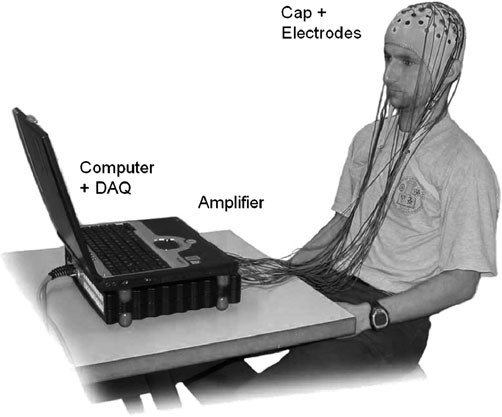
\includegraphics[width=70mm]{images/figure-2-1.jpg}
    \caption{Person records BCI data}
    \label{fig:my_label}
\end{figure}


\subsection{Processes of Operation}
BCI goes through three main procedures, measuring the brain activity, processing it and controlling the intercepted signals.
\subsubsection{Measuring Brain Activity}
Brain activity produces magnetic and electrical waves. That’s why, sensors or electrodes are used to measure these changes at different areas and times. Brain activities can be recorded through sensors (non-surgical solution) or electrodes (surgical solutions). For the non-surgical solution, sensors are used to measure the electrical activity from the scalp and this solution is called Electroencephalography (EEG) (Figure 2.1). They are relatively easy to deal with however they don’t provide accurate measures due to external interference and are susceptible to limitations in frequency range. In order to get consistent recording, sensors are spread on the scalp through system called 10 - 20 (Figure 2.2). 10 - 20 refers to how sensors are spread 10 - 20 - 20 - 20 - 20 - 10 percent. The 6 regions are named according to their position: Fp - pre-frontal, F - frontal, C - central, P - parietal, O - occipital, T - temporal. On the other hand, the surgical solution need to open the skull through surgical procedures and plant the electrodes. When the electrodes are planted on the surface of the cortex, it’s called electrocorticogram (ECoG). And another solution called Intracortical, which plants the electrodes in the inner parts of the brain. Although the surgical solutions provide higher accuracy and frequency range compared to the non-surgical solution they have serious drawbacks such as they need surgery, finance and can have ethical problems. Difference between each solution is shown in Figure 2.3.
\begin{figure}
    \centering
    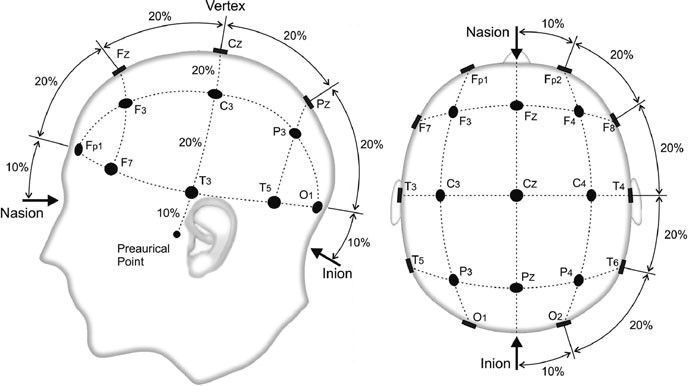
\includegraphics[width=70mm]{images/figure-2-2.jpg}
    \caption{10 - 20 System that shows how sensors are spread on the scalp}
    \label{fig:my_label}
\end{figure}
\begin{figure}
    \centering
    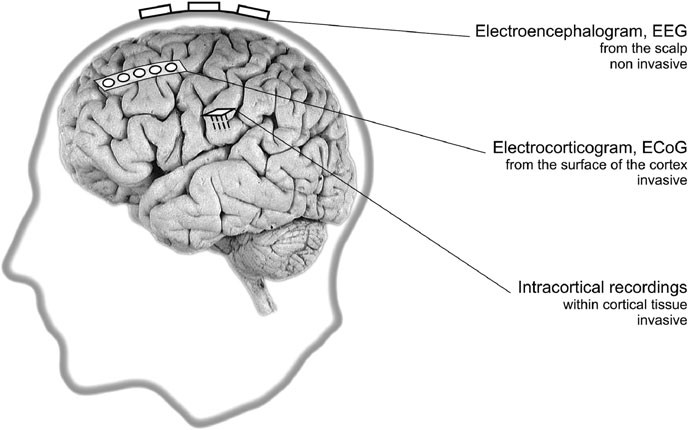
\includegraphics[width=70mm]{images/figure-2-3.jpg}
    \caption{Types of Reading Brain Waves on Computers (BCIs)}
    \label{fig:my_label}
\end{figure}

\subsubsection{Process and Control}
Processing and Controlling Received Signals are handled within the application.

\subsection{Brain Patterns}
Because measuring brain activity is not enough, some mental strategies are used to trigger the required tasks. The most used mental strategies are selective attention and motor imagery.
\subsubsection{Selective Attention}
Mental strategies based on selective attention require external stimuli such as auditory stimuli or visual stimuli. P300 (Peak signal at 300ms) or SSVEP (Steady-State Visual Evoked Potentials) are two mental strategies the depends on visual stimulation. P300 is triggered when the intensity of symbols is changed and SSVEP is triggered with flickering some areas with certain frequencies (6 – 30Hz).


\section{Online Dataset}
BCI2000, Competition III, Dataset II.

\subsection{Paradigm}
The user was shown a 6 by 6 matrix containing English letters and numbers (Figure 2.4). The user was to spell words and focus his attention of the character that he wants to choose. All rows and columns were intensified randomly and successively at a rate of 5.7Hz (100ms intensification, 75ms no intensification). In other words, a column or row is intensified (i.e. row 2 in Figure 2.4) for 100ms then, no row or column is intensified for 75ms, then repeat. The row and column (2 intensifications) which contained the chosen character will provide different signals (P300) compared to the other 10 intensifications which does not contain the chosen character (Non-P300).
\begin{figure}
    \centering
    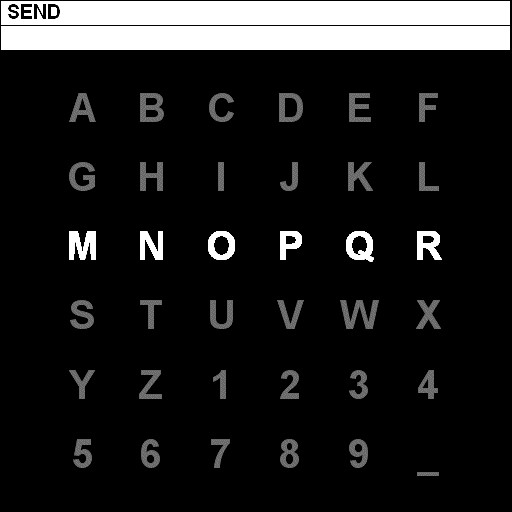
\includegraphics[width=70mm]{images/figure-2-4.jpg}
    \caption{The matrix displayed to the user}
    \label{fig:my_label}
\end{figure}

\subsection{Collection of Dataset}
Signals are filtered from 0.1 – 60Hz and digitized at 240Hz (Each 240 samples corresponds to 1 second). The 12 sets of intensifications were repeated 15 times for each character resulting in 180 total intensifications per epoch (character) into 64 channels EEG (Figure 2.5).
\begin{figure}
    \centering
    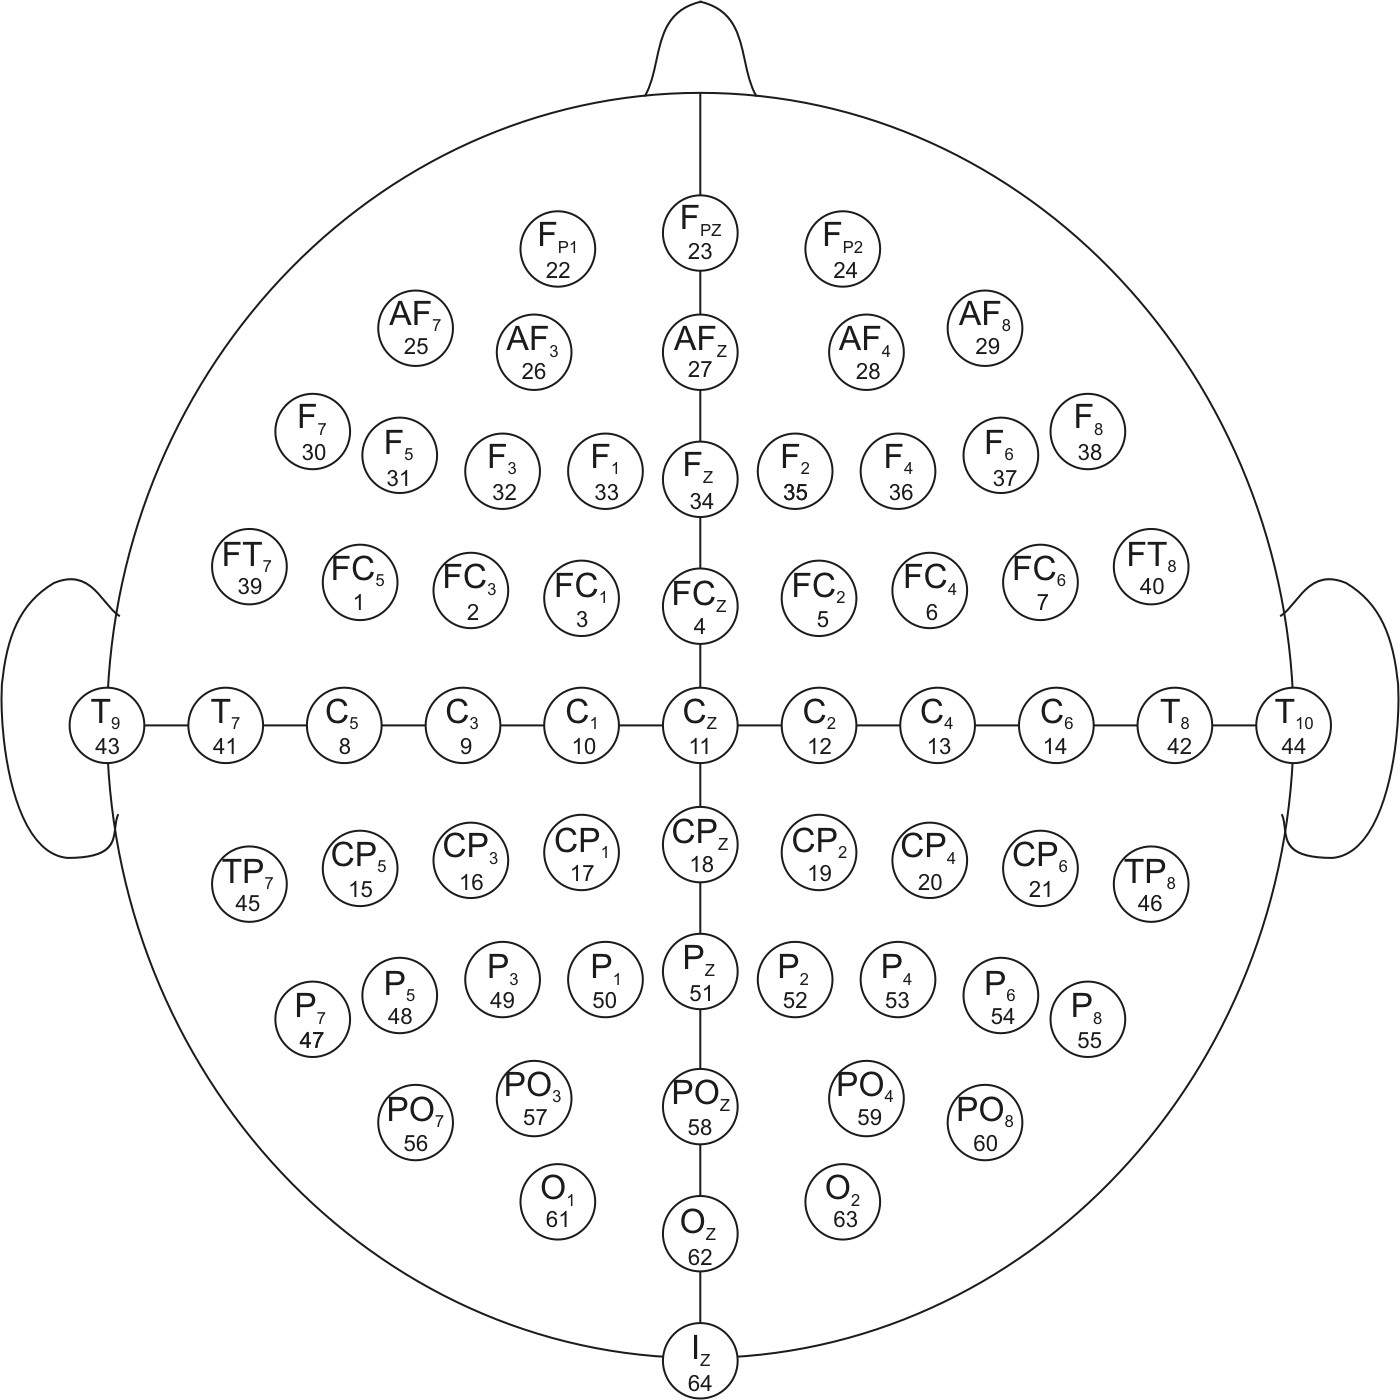
\includegraphics[width=70mm]{images/figure-2-5.jpg}
    \caption{Mapping of each sensors to its place on the scalp}
    \label{fig:my_label}
\end{figure}

\subsection{Explanation of The Dataset}
The dataset has 2 subjects (A and B), where each subject has 85 characters (epochs) in training dataset and 100 characters in testing dataset (Remember that, each epoch has 12 intensifications and 15 repetitions). The structure of variables for each subject file is described below.\newline
\begin{tabbing}
Title:\quad \quad \quad \quad \quad \=Description\kill
Signal:         \>signal of each channel (Figure 2.5)\\
                \>Type: 3D Array\\
                \>Shape (Dimension): (85, 7794, 64)\\
\newline\\
TargetChar:     \>The chosen character for each epoch\\
                \>Type: String\\
                \>Length: 85\\
\newline\\
Flashing:	    \>0	when NO row/column is intensified\\
                \>1	when row/column is intensified\\
                \>Type: 2D Array\\
                \>Shape (Dimension): (85, 7794)\\
\newline\\
StimulusCode:	\>0	when NO row/column is intensified\\
                \>1 ... 6	when intensified column (1 is left-most column)\\
                \>7 ... 12	when intensified row (1 is upper-most row)\\
                \>Type: 2D Array\\
                \>Shape (Dimension): (85, 7794)\\
\newline\\
StimulusType:	\>0	when NO row/column is intensified\\
		        \>1	when row/column contains the chosen character\\
                \>Type: 2D Array\\
                \>Shape (Dimension): (85, 7794)\\
\end{tabbing}
Note: 7794 samples because the data is digitized and there is a no-intensification period between each intensification.
Note: TargetChar, StimulusType are only provided for training dataset.

\subsection{Analysis}
Figure 2.6 shows signal wave forms for P300.
\begin{figure}
    \centering
    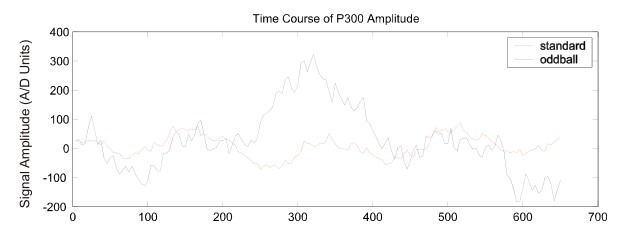
\includegraphics[width=70mm]{images/figure-2-6.jpg}
    \caption{Caption}
    \label{fig:my_label}
\end{figure}

